\documentclass[12pt,oneside]{book}
\usepackage{geometry}                		
\geometry{a4paper}                   			
    		
\usepackage{graphicx}				
									
\usepackage{amssymb}

\usepackage[spanish]{babel}			
\usepackage[utf8]{inputenc}			
\usepackage[T1]{fontenc}				
\usepackage{hyperref}				

\title{Proyecto Sudoku}
\author{Alvaro Ortiz\\ Denisse Pintado\\ Keyla Figueroa}
						

\begin{document}
\maketitle
\tableofcontents

\chapter{Introducción}
Este proyecto a sido implementado con la herramienta Qt en el lenguaje C++.Este juego ha sido desarrollado por el grupo Sudoku de la materia Lenguajes de Programación, ha sido implementado con las reglas del popular  juego matematico Sudoku, implementando algortimos para el llenado de los tableros en  los diferentes niveles y añadiendo ademas ayudas para el usuario que se anime a probar este maravilloso juego implementado de la manera mas original posible y siendo un producto elaborado con fines academicos.En el desarrollo de este manual daremos a conocer como se manejan los botones y que significan los controles que encontraremos en el transcurso del juego ademas, podremos entender mejor los comandos implementados en este juego y donde encontraras la ayuda en los diferentes niveles.Tambien se explicaran una que otra funciones para aquellos mas curiosos que deseen modificar codigo y crear su propio juego usando herramientas que talvez les sirvan para hacer algo mucho mas grande.

\chapter{Programa Sudoku}

En este manual empezaremos por explicar la pantalla de inicio como se muesta en la figura  \ref{Pantalla Inicial} la cual consta con el logo del Sudoku y con 3 opciones que son los niveles de dificultad a escoger Easy, Medium y Hard. Se debera seleccionar uno y acontinuacion aplastar el boton de Play, una vez que se seleccione la dificultad dara paso a la pantalla segun el nivel que escogio el usuario, se notara que en el caso de seleccionar play sin seleccionar una opcion se mostrara una  pantalla avisando del error como se muestra en esta imagen \ref{Pantalla Error}. Una vez que pasamos a la ventana que escogimos podemos empezar el juego con normalidad.

\begin{figure}[htbp]
\begin{center}
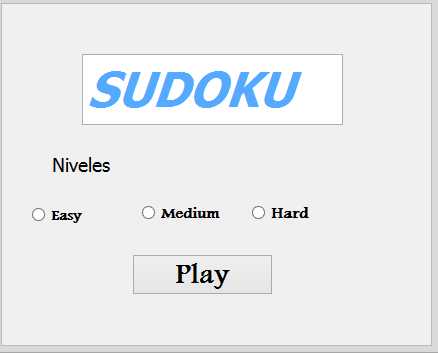
\includegraphics[width=.60\textwidth]{./imagenes/Pantalla Inicial.png}
\caption{Pantalla Inicial}
\label{Pantalla Inicial}
\end{center}
\end{figure}

\begin{figure}[htbp]
\begin{center}
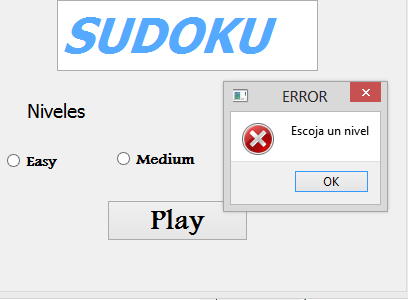
\includegraphics[width=.60\textwidth]{./imagenes/error.png}
\caption{Pantalla Error}
\label{Pantalla Error}
\end{center}
\end{figure}

Una vez que se selecciono el nivel de dificultad y se da clik al boton play podemos pasar a  explicar cada nivel. En el nivel Easy podemos observar en la figura   \ref{PantallaEasy} que tenemos 30 casillas llenas lo que facilitara resolver el tablero.En el caso de escoger el nivel de dificultad Medium\ref{PantallaSeleccionMedium} se tendran 25 casillas llenas en donde segun al algoritmo esto dara una dificultades extras en el juego como vemos en la figura \ref{PantallaMedium}  , ahora en el caso de escoger Nivel de dificultad  Hard tenemos una pantalla similar a la que se muestra en la figura \ref{PantallaHard} con tan solo 18 casillas llenas, en este caso el algoritmo que genera los numeros en el tablero se llena con el menor numero de numeros y este complica la resolución del tablero Sudoku.

\begin{figure}[htbp]
\begin{center}
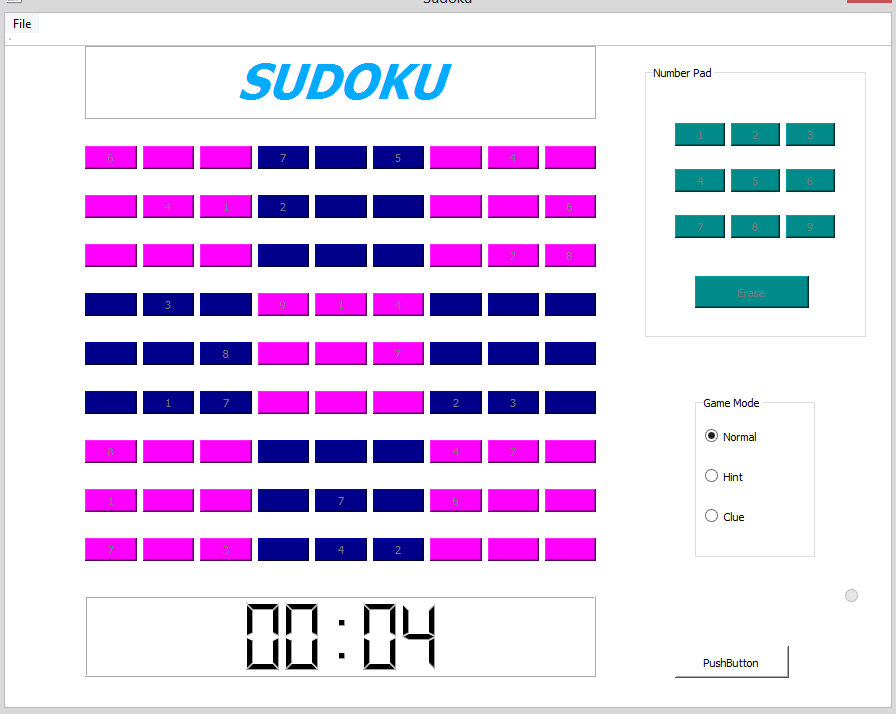
\includegraphics[width=.60\textwidth]{./imagenes/PantallaEasy.png}
\caption{PantallaEasy}
\label{PantallaEasy}
\end{center}
\end{figure}

\begin{figure}[htbp]
\begin{center}
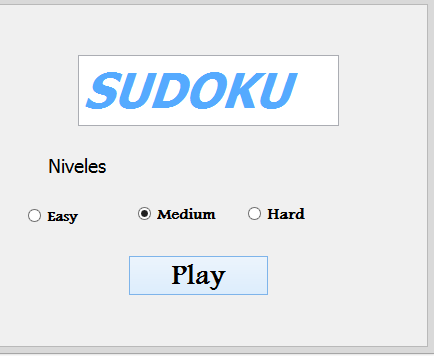
\includegraphics[width=.60\textwidth]{./imagenes/PantallaSeleccionMedium.png}
\caption{PantallaSeleccionMedium}
\label{PantallaSeleccionMedium}
\end{center}
\end{figure}

\begin{figure}[htbp]
\begin{center}
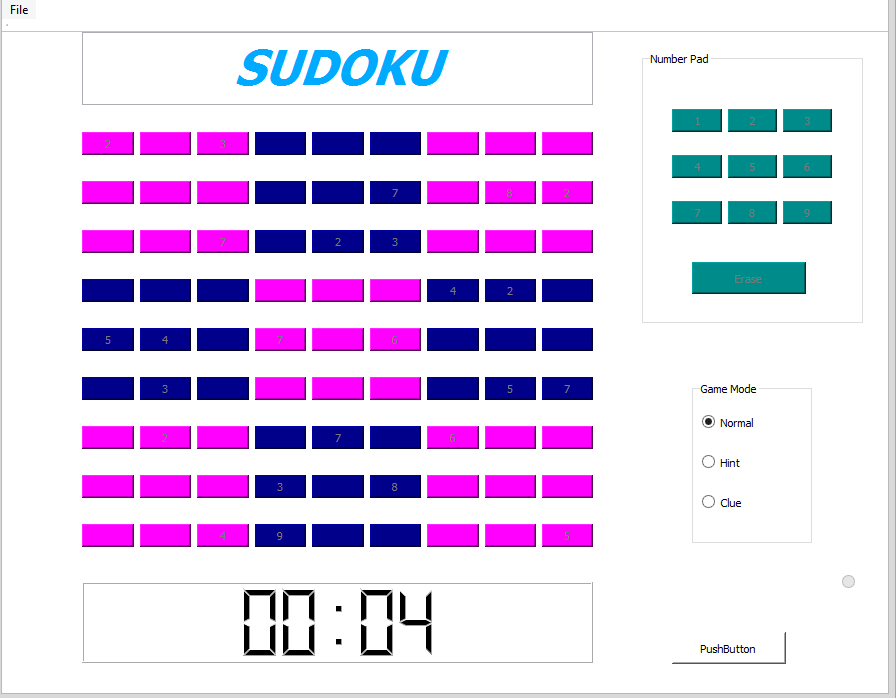
\includegraphics[width=.60\textwidth]{./imagenes/PantallaMedium.png}
\caption{PantallaMedium}
\label{PantallaMedium}
\end{center}
\end{figure}

\begin{figure}[htbp]
\begin{center}
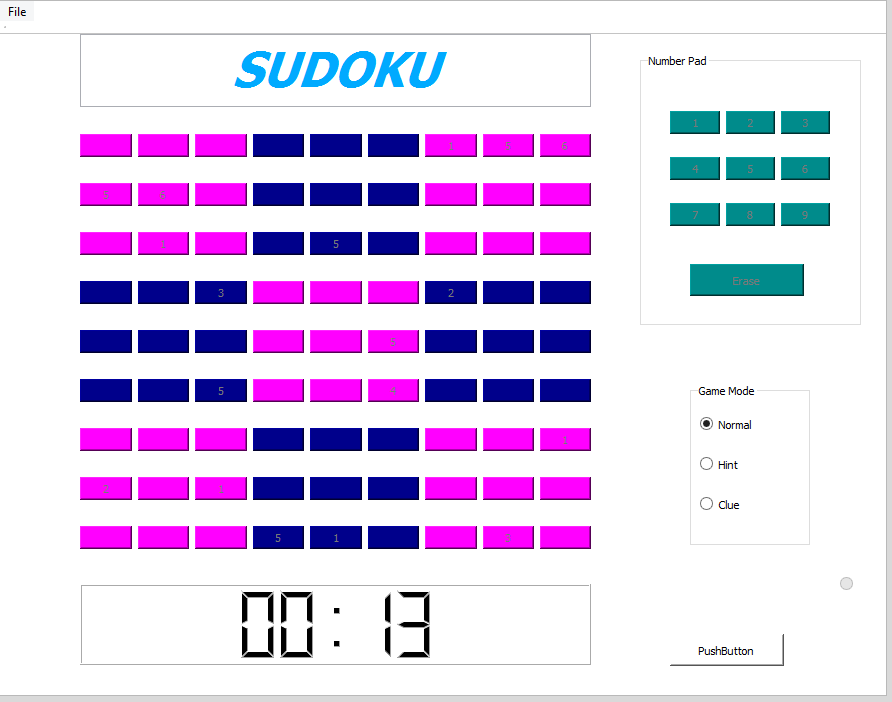
\includegraphics[width=.60\textwidth]{./imagenes/PantallaHard.png}
\caption{PantallaHard}
\label{PantallaHard}
\end{center}
\end{figure}

Ahora se explicara el GameMode que es la ayuda para el usuario, esta ayuda esta disponible en todo momento en cada una de la tres dificultades cuando el usuario quiera acceder a ella solo debera ubicarse en la parte inferior izquierda como se muestra en la figura \ref{dificultades} y escoger la que desee.


\begin{figure}[htbp]
\begin{center}
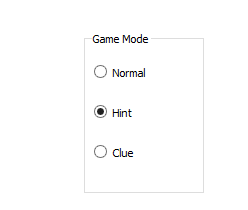
\includegraphics[width=.60\textwidth]{./imagenes/dificultades.png}
\caption{dificultades}
\label{dificultades}
\end{center}
\end{figure}

Explicando cada una de ellas en el caso de el modo de juego Normal la ayuda del usuario es quitada y solo se le da retroalimentación cambiando de color la celda que se encuentra seleccionada por el usuario al dar click en ella.Ahora esta modo esta habiliado por default es decir siempre funciona como primera instancia, cuando se habilite el modo Hint se podra notar una  ahora si una gran ayuda que hace que el usuario no se equivoque en todo el juego, cuando esta seleccionada esta casilla Hint lo que hace es deshabilitar en el NumberPad  \ref{NumberPad} todos los numeros que no serian posibles en la casilla seleccionada por conflictos en fila, columna o subtablero  como se muestra en la siguiente imagen.El juego tambien cuenta con un cronometro al inciar el juego comienza a funcionar


\begin{figure}[htbp]
\begin{center}
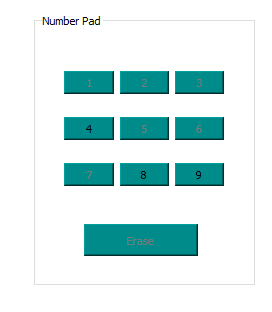
\includegraphics[width=.60\textwidth]{./imagenes/NumberPad.png}
\caption{NumberPad}
\label{NumberPad}
\end{center}
\end{figure}

\begin{figure}
\begin{center}
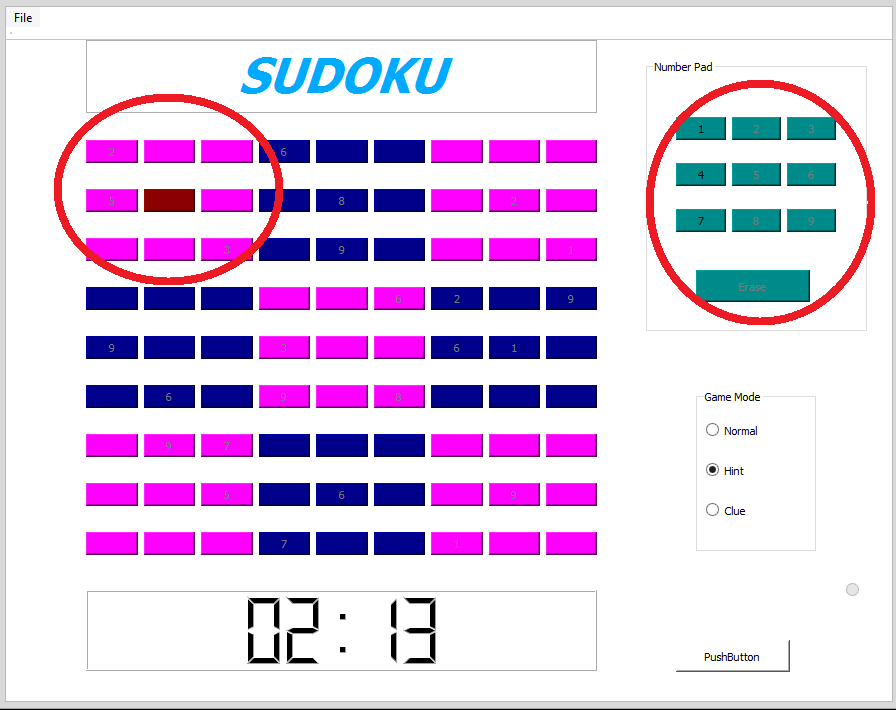
\includegraphics[width=.60\textwidth]{./imagenes/pantalla4.png}
\caption{Hint}
\label{Hint}
\end{center}
\end{figure}

\begin{figure}
\begin{center}
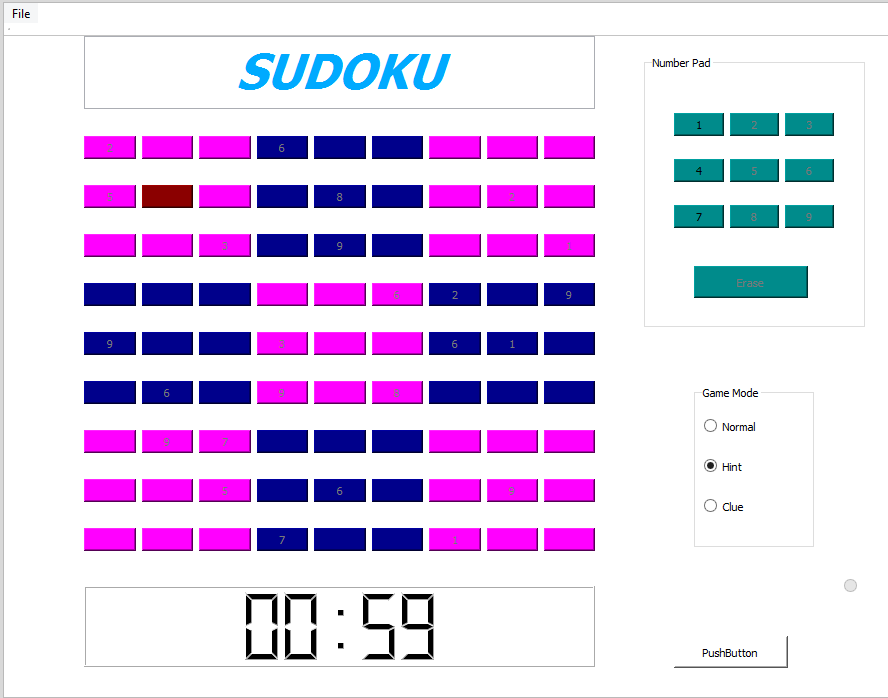
\includegraphics[width=.60\textwidth]{./imagenes/pantalla3.png}
\caption{Game Mode Normal}
\label{Game Mode Normal}
\end{center}
\end{figure}


\begin{figure}
\begin{center}
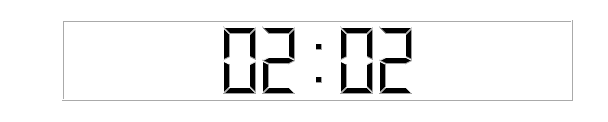
\includegraphics[width=.60\textwidth]{./imagenes/cronometro.png}
\caption{cronometro}
\label{cronometro}
\end{center}
\end{figure}



\begin{figure}[htbp]
\begin{center}
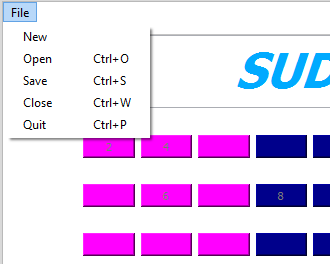
\includegraphics[width=.60\textwidth]{./imagenes/opciones.png}
\caption{opciones}
\label{opciones}
\end{center}
\end{figure}



\chapter{Conclusiones}
Se desarrollo este manual con el afán de explicar la funcionalidad del juego de una manera detallada para mas información del codigo se puede acceder a el manual generado por Doxygen o a la pagina html generada por el mismo donde se explican las funciones , formulas y maneras en las que se pudo implemtar este Juego.Esperando haya servido de una guia se propone a usted como usuario revisar las otras guias para expandir si conocimiento de como fue hecha esta aplicación.

\end{document}  
